\documentclass[12pt]{article}
\usepackage{amsfonts, amstext, amsmath, amsthm, amscd, amssymb, hyperref, float, longtable, fullpage}
\usepackage{epsfig, graphics, psfrag}
\usepackage{graphicx}
\graphicspath{ {images/} }
\usepackage[usenames,dvipsnames]{color}
\usepackage[font=small, labelfont=bf]{caption}
\usepackage{float}
\usepackage{mathrsfs}
\usepackage{mathtools}
\usepackage{tabto}
\usepackage{cite}
\usepackage{listings}
\usepackage{wrapfig}

\DeclareMathOperator{\Tr}{Tr}

\def\arraystretch{1.5}

\lstset{ 
  language=R,                     % the language of the code
  basicstyle=\ttfamily, % the size of the fonts that are used for the code
  numbers=left,                   % where to put the line-numbers
  numberstyle=\tiny\color{Blue},  % the style that is used for the line-numbers
  stepnumber=1,                   % the step between two line-numbers. If it is 1, each line
                                  % will be numbered
  numbersep=5pt,                  % how far the line-numbers are from the code
  backgroundcolor=\color{white},  % choose the background color. You must add \usepackage{color}
  showspaces=false,               % show spaces adding particular underscores
  showstringspaces=false,         % underline spaces within strings
  showtabs=false,                 % show tabs within strings adding particular underscores
  frame=single,                   % adds a frame around the code
  rulecolor=\color{black},        % if not set, the frame-color may be changed on line-breaks within not-black text (e.g. commens (green here))
  tabsize=2,                      % sets default tabsize to 2 spaces
  captionpos=b,                   % sets the caption-position to bottom
  breaklines=true,                % sets automatic line breaking
  breakatwhitespace=false,        % sets if automatic breaks should only happen at whitespace
  keywordstyle=\color{RoyalBlue},      % keyword style
  commentstyle=\color{YellowGreen},   % comment style
  stringstyle=\color{ForestGreen}      % string literal style
} 


\lstset{ 
  language=Python,                     % the language of the code
  basicstyle=\ttfamily, % the size of the fonts that are used for the code
  numbers=left,                   % where to put the line-numbers
  numberstyle=\tiny\color{Blue},  % the style that is used for the line-numbers
  stepnumber=1,                   % the step between two line-numbers. If it is 1, each line
                                  % will be numbered
  numbersep=5pt,                  % how far the line-numbers are from the code
  backgroundcolor=\color{white},  % choose the background color. You must add \usepackage{color}
  showspaces=false,               % show spaces adding particular underscores
  showstringspaces=false,         % underline spaces within strings
  showtabs=false,                 % show tabs within strings adding particular underscores
  frame=single,                   % adds a frame around the code
  rulecolor=\color{black},        % if not set, the frame-color may be changed on line-breaks within not-black text (e.g. commens (green here))
  tabsize=2,                      % sets default tabsize to 2 spaces
  captionpos=b,                   % sets the caption-position to bottom
  breaklines=true,                % sets automatic line breaking
  breakatwhitespace=false,        % sets if automatic breaks should only happen at whitespace
  keywordstyle=\color{RoyalBlue},      % keyword style
  commentstyle=\color{YellowGreen},   % comment style
  stringstyle=\color{ForestGreen}      % string literal style
} 


\def\layersep{2.5cm}

\newtheorem{definition}{Definition}[section] 
\let\olddefinition\definition
\renewcommand{\definition}{\olddefinition\normalfont}
\newtheorem{remark}{Remark}[section]
\let\oldremark\remark
\renewcommand{\remark}{\oldremark\normalfont}
\newtheorem{proposition}{Proposition}[section]
\newtheorem{theorem}{Theorem}[section]
\newtheorem{lemma}{Lemma}[section]
\newtheorem{corollary}{Corollary}[section]
\newtheorem{question}{Question}[section]
\newtheorem{notation}{Notation}[section]
\newtheorem{claim}{Claim}[section]
\newtheorem{example}{Example}[section]
\let\oldexample\example
\renewcommand{\example}{\oldexample\normalfont}

\newcommand{\catname}[1]{{\normalfont\textbf{#1}}}
\newcommand{\Set}{\catname{Set}}
\newcommand{\Rel}{\catname{Rel}}
\newcommand{\CRing}{\catname{CRing}}
\newcommand\opcat[1]{{#1}^{\mathrm{op}}}

\renewcommand{\baselinestretch}{1.5}

\begin{document}
\pagestyle{plain}
\begin{center}
STAT 4188 - Statistical Deep Learning  \hfill John Bochicchio and Anthony Shaw \\
Final Project \hfill  Due on 5/9/2019
\end{center}
\section{Results Report}
\tab For our project, we decided to compile our own dataset to use in exploring the future of the S\&P 500. Originally, our intent was to consider a number of macroeconomic variables and try and determine their effect on the business cycle, but we found this task far more difficult than we had thought. The datasets available to us were far too small (data was taken quarterly, which left us with less than 100 data points even over a long span of time), and many of the predictors varied wildly in their classification. As such, we decided to focus on the effects of one particular macroeconomic indicator (the 10 year treasury constant maturity or T10Y2Y for short) on the closing value of the S\&P 500. We wanted to attempt to predict fluctuations in the closing value of the S\&P 500, as well as understand the effects the 10 year treasury constant maturity had. We first compiled 16 years of both S\&P 500 and 10 year treasury constant maturity data.

\begin{figure}[H]
\centering
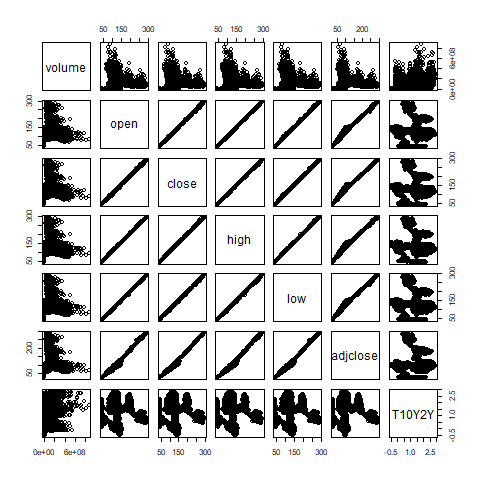
\includegraphics[scale=.5]{images/SPY-pairs.png}
\caption{Pairs for all values in our data set.}
\end{figure}

    The data sets considered were merged by timestamp, and any observations that had inconsistent or missing values were trimmed. This data merging and cleaning was done in Excel. We considered a number of methods before settling on our final approach. First, we looked at the pairs in our data set to try and determine what approaches might be useful. We found that most of the predictors shared a linear relationship, but the relationship between T10Y2Y and the closing price was more complex. We thought that perhaps a polynomial function might do a good job at approximating. We used cross validation and compared polynomial models of degrees between 1 and 4. We looked for the model with minimal error, which happened to be a polynomial of degree 3. This model had an MSE of .276, which is relatively good given the data set we were working with. We were able to get comparable results using a PCR model with cross validation, giving us an MSE of .287. We also attempted to fit a ridge regression to our data set. We first optimized our lambda parameter, but were unable to achieve acceptable results. Finally, we computed the persistent homology of our dataset and generated a barcode. 
    
\begin{figure}[H]
\centering
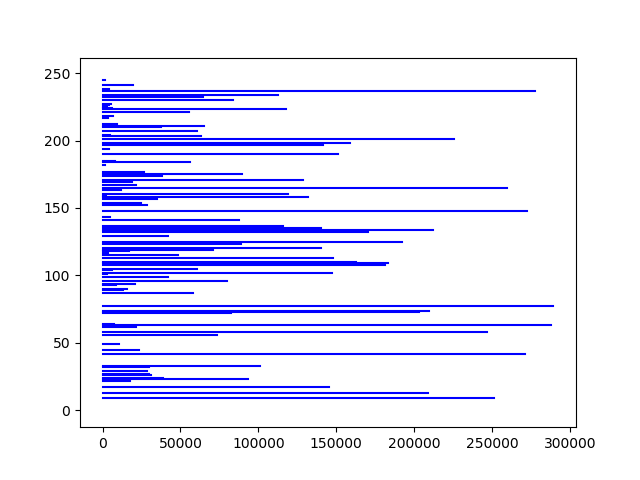
\includegraphics[scale=.75]{images/SPY-barcode.png}
\caption{Persistent homology barcode for the data set.}
\end{figure}
    
Persistent homology is useful in finding holes in datasets, and can sometimes allow one to reduce the dimension. The persistent homology barcode computed did not give easily interpretable results, and a large number of 2-holes were identified in the data that we were unable to smooth. Ultimately, we decided on a radial basis function network.
    
    Radial basis functions may be used in back-propagation neural networks, where the RBFs are essentially used as activators. Neural networks are universal approximators, and as such we know that given an activation function that satisfies certain conditions, any function can be approximated on a compact subset of real n-space using a single layer. We decided on radial basis functions as our activators due to their simplicity and fairly popular use in time-series analysis. Initially, we created a one layer RBF network, in which we calculated the weights through linear regression. This process is very simple, as it is essentially linear regression. First, we created our RBF, $\varphi(r)=e^{-(\varepsilon r)^{2}}$, where $\varepsilon$ is some scaling parameter, and $r$ is the norm  $\left\|\mathbf{x}-\mathbf{x}_{i}\right\|$. We calculate the interpolation matrix, 
$$S=
 \left[ \begin{array}{cccc}{\varphi\left(\left\|\mathbf{x}_{1}-\mathbf{x}_{1}\right\|\right)} & {\varphi\left(\left\|\mathbf{x}_{2}-\mathbf{x}_{1}\right\|\right)} & {\dots} & {\varphi\left(\left\|\mathbf{x}_{n}-\mathbf{x}_{1}\right\|\right)} \\ {\varphi\left(\left\|\mathbf{x}_{1}-\mathbf{x}_{2}\right\|\right)} & {\varphi\left(\left\|\mathbf{x}_{2}-\mathbf{x}_{2}\right\|\right)} & {\dots} & {\varphi\left(\left\|\mathbf{x}_{n}-\mathbf{x}_{2}\right\|\right)} \\ {\vdots} & {\vdots} & {\ddots} & {\vdots} \\ {\varphi\left(\left\|\mathbf{x}_{1}-\mathbf{x}_{n}\right\|\right)} & {\varphi\left(\left\|\mathbf{x}_{2}-\mathbf{x}_{n}\right\|\right)} & {\dots} & {\varphi\left(\left\|\mathbf{x}_{n}-\mathbf{x}_{n}\right\|\right)}\end{array}\right]$$

From here, it is a linear regression, in which we are solving for the weights $w_i$. Because RBF’s can approximate a function $y(x),$ in the form  $$y(\mathbf{x})=\sum_{i=1}^{N} w_{i} \varphi\left(\left\|\mathbf{x}-\mathbf{x}_{i}\right\|\right)$$ (where $N$ is the number of RBF’s) we can obtain the weights by calculating the matrix multiplication of the pseudo-inverse of S and the target values, $y(x).$ However, one of the issues with RBF’s, despite their fairly accurate interpolations, is that extrapolation is typically poor. 
    To try recover the accuracy of interpolation when performing time series prediction, we utilized the Gaussian RBF within a neural network containing 1 hidden layer and an arbitrary number of nodes $N$.

\newpage
\section{Technical Appendix}
The following R code was used for our initial exploratory analysis.
\begin{lstlisting}[language=R]
# Load CSV into data frame

SPY = read.csv(file="SPY.csv", header=T, sep=",")

# Drop date column and cast SPY
drop = c("date")
SPY = SPY[ , !(names(SPY) %in% drop)]

# Summarize inputs - sanity check
summary(SPY)

# Consider pairs
png("plot.png")
pairs(SPY)
dev.off()

# 65/35 test train split
sample <- sample(nrow(SPY), nrow(SPY)*.65, replace=F)
SPY.train <- SPY[sample,]
SPY.test <- SPY[-sample,]

# Initial linear model for calibration
SPY.lm <- lm(close ~ ., data=SPY.train)
SPY.lm.preds <- predict(SPY.lm, SPY.test)

mean((SPY.lm.preds - SPY.test$close)^2) #MSE

# Lambda optimized ridge regression
SPY.test.AsMatrix <- model.matrix(close ~ ., data=SPY.test)
SPY.train.AsMatrix <- model.matrix(close ~ ., data=SPY.train)

lambdaVal <- 10^seq(4,-2,length=100)

require(glmnet)

SPY.ridgeReg <- glmnet(SPY.train.AsMatrix, SPY.train$close, alpha=0, lambda=lambdaVal, thresh=1e-10)
SPY.crossRidge <- cv.glmnet(SPY.train.AsMatrix, SPY.train$close, alpha=0, lambda=lambdaVal, thresh=1e-10)

optimalLambda <- SPY.crossRidge$lambda.min
ridgePreds <- predict(SPY.ridgeReg, s=optimalLambda, newx=SPY.test.AsMatrix)

mean((ridgePreds - SPY.test$close)^2) #Get Ridge MSE

# PCR model
require(pls)

SPY.pcr <- pcr(close ~ ., data=SPY.train, scale=TRUE, validation="CV")
SPY.pcr.preds <- predict(SPY.pcr, SPY.test, ncomp=6)

mean((SPY.pcr.preds - SPY.test$close)^2)
\end{lstlisting}

We also used the Dionysus Python package to compute the persistent homology groups of the data.

\begin{lstlisting}[language=Python]
import dionysus._dionysus as d
import dionysus.plot as plot
import matplotlib.pyplot as plt
import numpy as np
import pandas as pd

# Import data and remove date column
SPY = pd.read_csv("SPY.csv")
SPY = SPY.iloc[:,1:].sample(250)
SPY = SPY.values

# Generate rips filtration
print("Generating Rips filtration...")
rips_filtration = d.fill_rips(SPY, 2, 300000)
print(rips_filtration)

# Compute the persistent homology of the filtration
print("Computing persistent homology of Rips filtration...")
persistence = d.homology_persistence(rips_filtration)
diag = d.init_diagrams(persistence, rips_filtration)

# Show the bar diagram
plot.plot_bars(diag[0], show = True)
\end{lstlisting}

Finally, we used the following Python code for the neural network:
\end{document}